%
% $File: report.tex
% $Date: Sun Nov 17 23:42:24 2013 +0800
%

\documentclass{article}
\usepackage{fontspec}
\usepackage{zhspacing,url,amsmath,amssymb,verbatim}
\usepackage{pdfpages}
\zhspacing
\usepackage{listings}
\usepackage[hyperfootnotes=false,colorlinks,linkcolor=blue,anchorcolor=blue,citecolor=blue]{hyperref}
\usepackage[backend=biber]{biblatex}
\usepackage{graphicx}
\usepackage{minted}
\usepackage{subfigure}
\usepackage{indentfirst}
\usepackage{cases}
\usepackage{environ}
\usepackage{array}
\usepackage[top=1in, bottom=1in, left=1.25in, right=1.25in]{geometry}
\usepackage{caption}
%\usepackage{tikz}
%\usepackage{dot2texi}

% $File: mint-defs.tex
% $Date: Thu Sep 26 22:11:33 2013 +0800
% $Author: Xinyu Zhou <zxytim@gmail.com>

\newcommand{\inputmintedConfigured}[3][]{\inputminted[fontsize=\footnotesize,
	label=#3,linenos,frame=lines,framesep=0.8em,tabsize=4,#1]{#2}{#3}}

\newcommand{\txtsrc}[2][]{\inputmintedConfigured[#1]{text}{#2}}
\newcommand{\txtsrcpart}[4][]{\txtsrc[firstline=#3,firstnumber=#3,lastline=#4,#1]{#2}}

\newcommand{\cppsrc}[2][]{\inputmintedConfigured[#1]{cpp}{#2}}
\newcommand{\cppsrcpart}[4][]{\cppsrc[firstline=#3,firstnumber=#3,lastline=#4,#1]{#2}}

\newcommand{\javasrc}[2][]{\inputmintedConfigured[#1]{java}{#2}}
\newcommand{\javasrcpart}[4][]{\javasrc[firstline=#3,firstnumber=#3,lastline=#4,#1]{#2}}

\newcommand{\matlabsrc}[2][]{\inputmintedConfigured[#1]{matlab}{#2}}
\newcommand{\matlabsrcpart}[4][]{\matlabsrc[firstline=#3,firstnumber=#3,lastline=#4,#1]{#2}}

%\usepackage[T1]{fontenc}
\usepackage{lmodern}
\usepackage{amssymb,amsmath}
\usepackage{ifxetex,ifluatex}
\usepackage{fixltx2e} % provides \textsubscript
% use upquote if available, for straight quotes in verbatim environments
\IfFileExists{upquote.sty}{\usepackage{upquote}}{}
\ifnum 0\ifxetex 1\fi\ifluatex 1\fi=0 % if pdftex
  \usepackage[utf8]{inputenc}
\else % if luatex or xelatex
  \usepackage{fontspec}
  % commented by Xinyu Zhou
  \ifxetex
    \usepackage{xltxtra,xunicode}
  \fi
  \defaultfontfeatures{Mapping=tex-text,Scale=MatchLowercase}
  \newcommand{\euro}{€}
\fi
% use microtype if available
\IfFileExists{microtype.sty}{\usepackage{microtype}}{}
\usepackage{color}
\usepackage{fancyvrb}
\newcommand{\VerbBar}{|}
\DefineShortVerb[commandchars=\\\{\}]{\|}
\DefineVerbatimEnvironment{Highlighting}{Verbatim}{commandchars=\\\{\}}
% Add ',fontsize=\small' for more characters per line
\newenvironment{Shaded}{}{}
\newcommand{\KeywordTok}[1]{\textcolor[rgb]{0.00,0.44,0.13}{\textbf{{#1}}}}
\newcommand{\DataTypeTok}[1]{\textcolor[rgb]{0.56,0.13,0.00}{{#1}}}
\newcommand{\DecValTok}[1]{\textcolor[rgb]{0.25,0.63,0.44}{{#1}}}
\newcommand{\BaseNTok}[1]{\textcolor[rgb]{0.25,0.63,0.44}{{#1}}}
\newcommand{\FloatTok}[1]{\textcolor[rgb]{0.25,0.63,0.44}{{#1}}}
\newcommand{\CharTok}[1]{\textcolor[rgb]{0.25,0.44,0.63}{{#1}}}
\newcommand{\StringTok}[1]{\textcolor[rgb]{0.25,0.44,0.63}{{#1}}}
\newcommand{\CommentTok}[1]{\textcolor[rgb]{0.38,0.63,0.69}{\textit{{#1}}}}
\newcommand{\OtherTok}[1]{\textcolor[rgb]{0.00,0.44,0.13}{{#1}}}
\newcommand{\AlertTok}[1]{\textcolor[rgb]{1.00,0.00,0.00}{\textbf{{#1}}}}
\newcommand{\FunctionTok}[1]{\textcolor[rgb]{0.02,0.16,0.49}{{#1}}}
\newcommand{\RegionMarkerTok}[1]{{#1}}
\newcommand{\ErrorTok}[1]{\textcolor[rgb]{1.00,0.00,0.00}{\textbf{{#1}}}}
\newcommand{\NormalTok}[1]{{#1}}
% \ifxetex
%   \usepackage[setpagesize=false, % page size defined by xetex
%               unicode=false, % unicode breaks when used with xetex
%               xetex]{hyperref}
% \else
%   \usepackage[unicode=true]{hyperref}
% \fi
\hypersetup{breaklinks=true,
            bookmarks=true,
            pdfauthor={},
            pdftitle={},
            colorlinks=true,
            urlcolor=blue,
            %linkcolor=magenta,
            pdfborder={0 0 0}}
%\urlstyle{same}  % don't use monospace font for urls
\setlength{\parindent}{0pt}
\setlength{\parskip}{6pt plus 2pt minus 1pt}
\setlength{\emergencystretch}{3em}  % prevent overfull lines
%\setcounter{secnumdepth}{0}



\newcommand{\figref}[1]{\hyperref[fig:#1]{Figure\ref*{fig:#1}}}
\newcommand{\tableref}[1]{\hyperref[table:#1]{Table\ref*{table:#1}}}
\newcommand{\centerize}[1]{\begin{center} #1 \end{center}}

\newcommand{\cmd}[1]{{\it #1}}
\newcommand{\ccmd}[1]{\centerize{\cmd{#1}}}

\title{Digital Signal Processing: Speaker Recognition \\ Progress Report}
\author{Xinyu Zhou, Yuxin Wu, and Tiezheng Li\\ Tsinghua University}
\date{}

\bibliography{refs.bib}
\begin{document}

\fontsize{11pt}{1.4em}
\setlength{\baselineskip}{1.6em}
\maketitle


\section{Introduction}
A \textbf{Speaker Recognition} tasks can be classified with respect to different criterion:
Text-dependent or Text-independent, Verification (decide whether the person is he claimed to be) or Identification (decide who the person is by its voice).\cite{SRwiki}

Speech is a kind of complicated signal produced as a result of several transformations occurring at different levels: semantic, linguistic and acoustic.
Differences in these transformations may lead to differences in the acoustic properties of the signals.
The recognizability of speaker can be affected not only by the linguistic message
but also the age, health, emotional state and effort level of the speaker.
Background noise and performance of recording device also interfere
the classification process.

Speaker recognition is an important part of Human-Computer Interaction (HCI).
As the trend of employing wearable computer reveals,
Voice User Interface (VUI) has been a vital part of such computer.
As these devices are particularly small, they are more likely to lose and be stolen.
In these scenarios, speaker recognition is not only a good HCI,
but also a combination of seamless interaction with computer and security guard
when the device is lost.
The need of personal identity validation will become more acute in the future.
Speaker verification may be essential in business telecommunications.
Telephone banking and telephone reservation services will develop rapidly
when secure means of authentication were available.

Also,the identity of a speaker is quite often at issue in court cases.
A crime victim may have heard but not seen the perpetrator,
but claim to recognize the perpetrator as someone whose voice was previously familiar;
or there may be recordings of a criminal whose identity is unknown.
Speaker recognition technique may bring a reliable scientific determination.

Furthermore, these techniques can be used in environment which demands high security.
It can be combined with other biological metrics to form a multi-modal authentication system.

In this task, our goal is to build a proof-of-concept text-dependent speaker recognition system with GUI support.
Hopefully, we would like to extend its ability to a text-independent speaker recognition system.

%File: algorithm.tex
%Date: Sun Nov 17 23:43:49 2013 +0800
%Author: Yuxin Wu <ppwwyyxxc@gmail.com>

\section{Algorithm and Implementation}

We presented a prototype system based on MFCC as acoustic features, and
GMM as our recognition model.

\subsection{MFCC}
MFCC (Mel-frequency Cepstral Coefficient) is a representation of the short-term power spectrum of a sound,
based on a linear cosine transform of a log
power spectrum on a nonlinear mel-scale of frequency \cite{mfcc} .
MFCC is the mostly widely used features in Automatic Speech Recognition(ASR), and it can also be
applied to Speaker Recognition task.

The process to extract MFCC feature is as followed:
\begin{figure}[H]
  \centering
  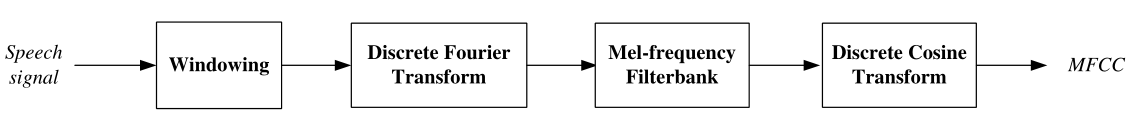
\includegraphics[width=\textwidth]{res/MFCC.png}
\end{figure}

First, the input speech should be divided into successive short-time frames of length $L$,
neighboring frames shall have overlap $R$. In our implementation, We choose $L = 20ms  $ ans $ R = 10 ms$.
Those frames are then windowed by Hamming Window, as shown in \figref{frames}
\begin{figure}[H]
  \centering
  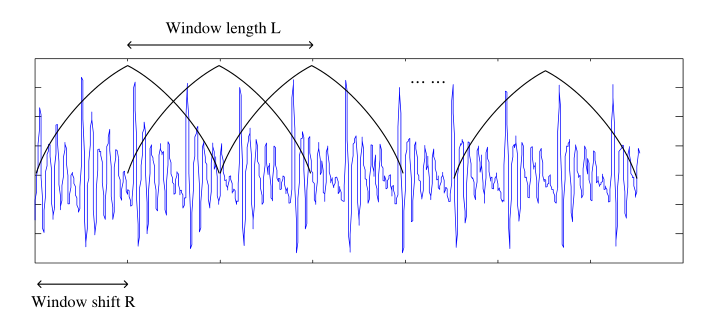
\includegraphics[width=0.7\textwidth]{res/frames.png}
  \caption{Framing and Windowing \label{fig:framming}}
\end{figure}

Then, We perform Discrete Fourier Transform (DFT) on windowed signals to compute their spectrums.
For each of $N$ discrete frequency bands we get a complex number $X[k]$ representing
magnitude and phase of that frequency component in the original signal.

Considering the fact that human hearing is not equally sensitive to all frequency bands, and especially, it has lower resolution at higher frequencies.
Scaling methods like Mel-scale and Bark-scale are aimed at scaling the frequency domain to fit human auditory perception better.
They are approximately linear below 1 kHz and logarithmic above 1 kHz.
\begin{figure}[H]
  \centering
  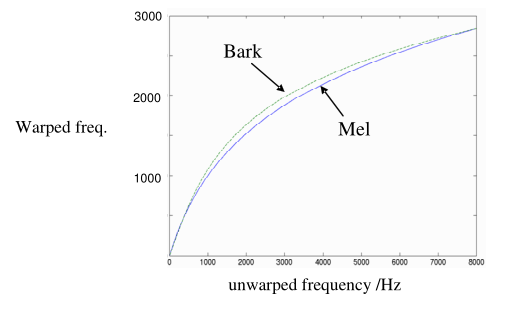
\includegraphics[width=0.6\textwidth]{res/mel-scale.png}
\end{figure}

In MFCC, Mel-scale is applied on the spectrums of the signals. The expression of Mel-scale warpping is as followed:
\[ M(f) = 2595 \log_{10}(1 + \dfrac{f}{700}) \]

\begin{figure}[H]
  \centering
  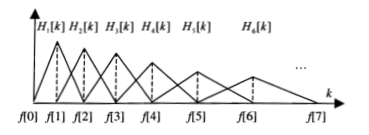
\includegraphics[width=0.5\textwidth]{res/bank.png}
  \caption{Filter Banks (6 filters) \label{fig:bank}}
\end{figure}
Then,  we appply the bank of filters according to Mel-scale on the spectrum,
calculate the logarithm of energy under each bank by $E_i[m] = \log (\sum_{k=0}^{N-1}{X_i[k]^2 H_m[k]}) $ and apply Discrete
Cosine Transform (DCT) on $E_i[m](m = 1, 2, \cdots M) $ to get an array $c_i $:
\[ c_i[n] = \sum_{m=0}^{M-1}{E_i[m]\cos(\dfrac{\pi n}{M}(m - \dfrac{1}{2}))} \]

Usually, the first 13 terms in $c_i $ is used as features for future training.

\subsection{GMM}

We use Gaussian Mixture Model (GMM) to model all features from one person.
For implementation, we use the GMM model training and predicting routine from the famous python
machine learning package scikit-learn \cite{sklearn}.
Since the last step of MFCC is DCT, different dimensions of the features are strongly independent, so we
use GMM with diagonal covariance matrix. The number of components in GMM is chosen as 32 in our implementation.

After building models for each person, it can be used to calculate the probability that the input signal is generated by this model.
The model with maximum probability is picked out as the result, and the corresponding person is recognized.

\pysrcpart{res/test.py}{45}{50}

\section{Test}
The corpus we use comprise of three different speakers: two men and one woman.
Each speaker has 460 samples, where the average duration of each sample is
about 4 seconds.  For each speaker, we randomly choose $M$ samples to train GMM
model. For more deep inspection of the algorithm, M is enumerated from 2 to 5.
We then feed the whole corpus to to the algorithm, and test its accuracy.
Further more, for the robustness of the result, we repeat the test process 10
times, and average the result.

\subsection{Result}
\begin{figure}[!ht]
\centering
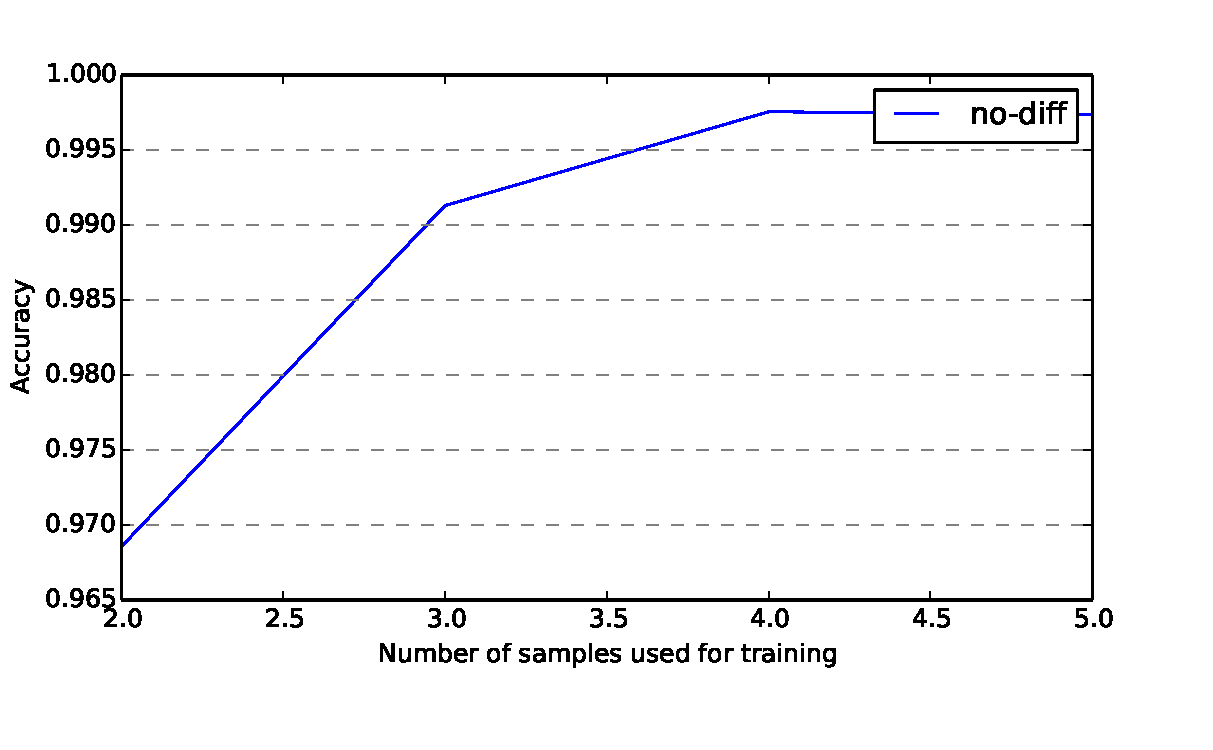
\includegraphics[width=\textwidth]{res/plot.pdf}
\caption{Accuracy vs Number of samples used for training}
\label{fig:result}
\end{figure}

\begin{table}[!ht]
	\centering
	\begin{tabular}{|c|c|c|c|c|}
		\hline
        \#Training sample & 2 & 3 & 4 & 5 \\\hline
		Accuracy & 0.968555 & 0.991293 & 0.997549 & 0.997380 \\\hline
	\end{tabular}
	\label{table:result}
\end{table}

As we can see from the curve ploted, the performance of the algorithm increases as
the number of training samples given increases. The accuracy when
just using two training samples for each user has reached $96.55\%$, which
is supprisingly high with respect to using such small amount of training samples.

When using 4 to 5 samples per speaker, the accuracy is above $99.73\%$, which
strongly confirmed the effectivenes of MFCC feature and GMM modeling for each
speaker.

However, further inspection on misclassified samples showed limitation on our
test case: all the misclassified samples are within two men speakers, indicates
the weakness of the algorithm.

\section{Future Work}

A text-independent speaker-recognition system is presented at this period.
But our current still have lots of limitations.
Due to our time devoted in, we only manage to acquire a small corpus on the Internet with only 3 people.
The data in the corpus is quite clear, thus we may need to do some further test on the robustness of our
algorithm.

In the future, we are focusing on variables in input limitation. The
recognizability of speaker can be affected not only by the linguistic message
but also the age, health, emotional state and effort level of the speaker.
Background noise and performance of recording device also interfere the
classification process.

A goal we want to achieve in this project can be described as follows: For a clear conversation signal between two persons, with no sentences
overlapped and significant interval between sentences, we may separate the conversation signal into two parts. Each part is exactly all the sentences
spoken by a certain speaker.

A main challenge is that MFCC's performance decreases incredibly when the strength of background noise enhances.  A series of speech noise reduction
algorithms needs to be applied on the input signals. Fortunately, much work in this field has been done previously. Spectral Subtraction(SS) that
incorporates noise over time, and SPLICE algorithm that makes no assumptions about noise stationarity can be applied to build a noise-robust
recognition system as two examples.
Another challenge settles in separating overlapped sentences from two or more different speakers.
Vocal separation is a challenging problem, to date
there is no general algorithm that ensures perfect separation effect.
Some commonly used models and algorithms are listed as follows: NSA, LVD/PLCA,
SFD, etc. More work on this field will be done till next period.

\printbibliography

\end{document}

